\chapter{Analyzing Merge-Conflict Resolutions}
In this section we describe how we analyzed merge-conflict resolutions. A manual analysis was conducted and the result of this, which is presented in the Result chapter, was used in an automatic analysis.
\section{Conflict File Tree}\label{sec:cft}
To get a better overview of how the different versions of a file look, we developed a tool to create a file tree of all conflicts of a given project. We call this file tree the Conflict File Tree. The leaves of the tree consist of the left-, right-, common ancestor- and merge commit version of a conflicting file when re-creating merge commits, as shown in Figure \ref{fig:cft}.

To do this, we first needed to find the two parents of a merge commit, that is, the two commits that were merged. The following command prints the two commits:
\lstset{language=Bash,numbers=left,xleftmargin=2em,frame=single,framexleftmargin=1.5em}
\begin{lstlisting}[frame=single,breaklines=true,tabsize=2]
git --no-pager log --merges --format=%p <hash> | head -n1
\end{lstlisting}
where <hash> is the merge commit hash. The two parent commits are hereby referred to as C1 and C2. We then re-create the merge using the following:
\lstset{language=Bash,numbers=left,xleftmargin=2em,frame=single,framexleftmargin=1.5em}
\begin{lstlisting}[frame=single,breaklines=true,tabsize=2]
git reset --hard <hash of C1>
git clean -f
git branch <temp branch name>
git checkout <hash of C2>
git merge <temp branch name>
\end{lstlisting}
In line 1, we set HEAD to commit C1, which changes the working copy to the state of that C1. In line 2,  the working copy is cleaned to be ready for the merge. In line 3, a new branch is created which points at commit C1. In line 4, we checkout commit C2. In line 5, we merge the two commits by merging the newly created branch into commit C2. Git will now print out the conflicting files, which we parse. Afterwards, we abort the merge and delete the branch.

The common ancestor-, local- and remote file, along with the resulting resolution file in the merge commit, are copied and saved in the Conflict file tree. The Conflict File Tree consist of folders and the versions of the conflicting files, structured according to Figure \ref{fig:cft}.\\
\begin{figure}[H]
\centering
%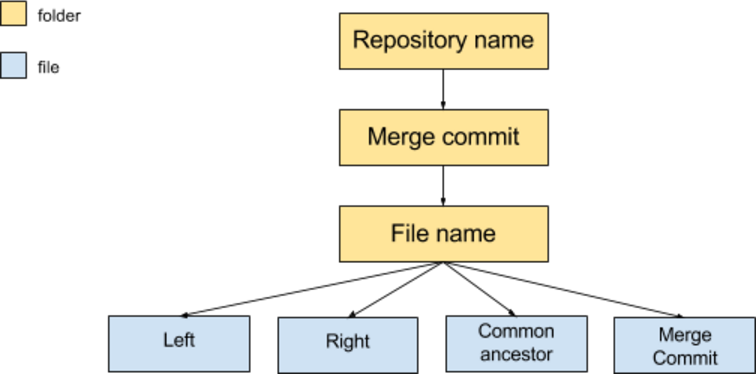
\includegraphics[width=0.45\linewidth, trim=3cm 11cm 3cm 11cm]{figure/conflicts.png}
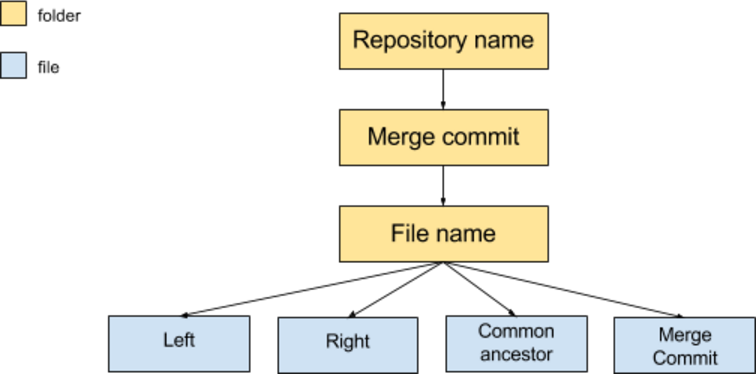
\includegraphics[width=400pt]{figure/conflicts.png}
\caption{Structure of a Conflict File Tree}\label{fig:cft}
\end{figure}

Having all the conflicting file versions in a structured manner made it easier to manually analyze how Git conflicts look like in files. To get the information about the conflict, we use following command:
\lstset{language=Bash,numbers=left,xleftmargin=2em,frame=single,framexleftmargin=1.5em}
\begin{lstlisting}[frame=single,breaklines=true,tabsize=2]
git merge-file -p --diff3 <left> <ancestor> <right>
\end{lstlisting}
The CFT was used in our manual analysis, see Section \ref{sec:manual}.
\section{Classify Merge-Conflicts}
To classify conflicts, we used the tool Conflicts Analyzer developed by Accioly. The tool produces a conflict report with information of each conflict of a specified project. We extended the tool to add additional information as follows; the merge commit hash, the parent 1 hash, and the parent 2 hash. Since the tool uses a merge technique different from that used in Git, it finds conflicts that are not a conflict in Git. As we are interested in how the developers themselves solve conflicts, we are not interested in these additional conflicts. Therefore we also modified the tool to only analyze conflicts from merges that also yield a conflict when merged by Git. We did this by reusing our code that re-creates merges (see Section \ref{sec:cft}).

The output in the conflict report contains the following information:
\begin{itemize}
\item Conflict type
\item Merge commit hash
\item Parent1 hash
\item Parent2 hash
\item Conflict body
\item File path
\end{itemize}

\section{Manual Analysis}\label{sec:manual}
\FloatBarrier
When manually analyzing the output of Conflicts Analyzer, we found that it may be possible to categorize the resolutions for the conflict pattern SameSignatureCM (see Table \ref{table:conflictpatterns}) by comparing the two conflicting versions with the resolution. This conflict pattern means that two versions was added for the same method or constructor, i.e the method did not exist in the common ancestor. 

We examined twenty-six randomly sampled examples of SameSignatureCM conflicts from 9 different projects. These projects were Atmosphere, Activiti, Blueprints, BroadLeadCommerce, Buildcraft, EventBus, android-async-http, RxJava, Elasticsearch. For each conflict, we looked at the two versions of the method or constructor, and tried to understand why they chose the one they did. What do the versions they chose have in common?

To categorize the merge-conflict resolutions, we proposed some categories which we wanted to test in a quantitative analysis. 
\begin{table}
\caption{Proposed categories}\label{table:pcategories}
\begin{tabular}{ p{7cm} p{7cm} }
\hline
\multicolumn{1}{c}{\textbf{Category}} & \multicolumn{1}{c}{\textbf{Description}}\\
Recent & The result is equal to the most recent version\\
Superset & The result is a superset of the code in both versions\\
Intersection & The result is an intersection of the code in both versions\\
\end{tabular}
\end{table}
\FloatBarrier
To be able to analyze conflicts from the output of Conflicts Analyzer, we wrote a Bash script to automatically extract the Java-files that conflicted in the merge, as well as the common ancestor file and the resolution file after the merge was made.

To extract the files, the script first resets the git repository so that HEAD points to the same commit as the latest commit on the remote master branch. Since the output from Conflicts Analyzer strip down the commit hash, our script parses the full commit hash of the parents from the git log. From the git log, the hash of the merge commit is also parsed. Using the git command:
\lstset{language=Bash,numbers=left,xleftmargin=2em,frame=single,framexleftmargin=1.5em}
\begin{lstlisting}[frame=single,breaklines=true,tabsize=2]
git --no-pager log --merges --format=%p <hash> | head -n1
\end{lstlisting}
where \textit{hash} is the merge commit hash. We then parse the two commits and perform the merge using the following sequence of commands:\\
\lstset{language=Bash,numbers=left,xleftmargin=2em,frame=single,framexleftmargin=1.5em}
\begin{lstlisting}[frame=single,breaklines=true,tabsize=2]
git merge-base <C1> <C2>
\end{lstlisting}
Where \textit{C1} and \textit{C2} refer to the hashes of the parents.  Then, the two parent commits, the merge commit, and the common ancestor commit are checked out respectively and the desired file is copied to a specified output folder. Finally, the script parses the date of the parent commits and prints it to a file in the specified output folder.

We analyzed the extracted files manually to see whether the categories described in Table \ref{table:pcategories} would emerge repeatedly in many resolutions. The data gathered in the manual analysis consisted of Project name, Function name, Merge hash, Merge commit message, Parent1 hash, Parent2 hash, Parent1 date, Parent2 date, Conflict pattern, Resolution categories, Comment. We also found out that we can apply these same proposed categories for the conflict pattern EditSameMC (see Table \ref{table:conflictpatterns}). For EditSameMC, the method existed in the common ancestor but was modified in both versions.
\FloatBarrier
\section{Automatic Analysis}
To see whether the results from the manual analysis still apply in a large-scale analysis, we developed a tool that reads the output of Conflicts Analyzer. The tool then filters out those conflicts we are interested in. Those conflicts are then analyzed and the result is printed in a spreadsheet.

From the qualitative analysis, we saw that sometimes the version that is chosen has more if-statements than the other version. We decided that it would be interesting to see whether choosing such a version reoccurs in many cases. It would also be interesting to see other cases where the version chosen had more of error handling and log printouts. Therefore, we proposed a list of keywords to search for in the versions. Thus, the complete list of categories we analyze is as shown in Table \ref{table:pcategories2}.
\begin{table}
\caption{Proposed categories}\label{table:pcategories2}
\begin{tabular}{ p{7cm} p{7cm} }
\hline
\multicolumn{1}{c}{\textbf{Category}} & \multicolumn{1}{c}{\textbf{Description}}\\
Recent & The result is equal to the most recent version\\
Superset & The result is a superset of the code in both versions\\
Intersection & The result is an intersection of the code in both versions\\
if & The result is equal to the version which contains most if-statements\\
print & The result is equal to the version which contains most instances of the keyword print\\
log & The result is equal to the version which contains most instances of the keyword log\\
try & The result is equal to the version which contains most instances of the keyword try\\
\end{tabular}
\end{table}

\subsection{Input}
We use the data from Conflicts Analyzer as input for our tool. As stated in Section \ref{sec:cp}, we are only interested in conflicts that are of the types SameSignatureCM or EditSameMC. Therefore, our tool filters out conflicts that are not of these patterns. It also removes conflicts in which any version of the function is empty, ie. the function was removed in one version. Conflicts that contain obscure output data from Conflicts Analyzer, such as if the conflict is not a git conflict, are also skipped.

Figure \ref{fig:screenshot} shows a screenshot of an example output from Conflicts Analyzer. The data surrounded by a red border are the data we use as input for our tool.
\begin{figure}[H]
\centering
%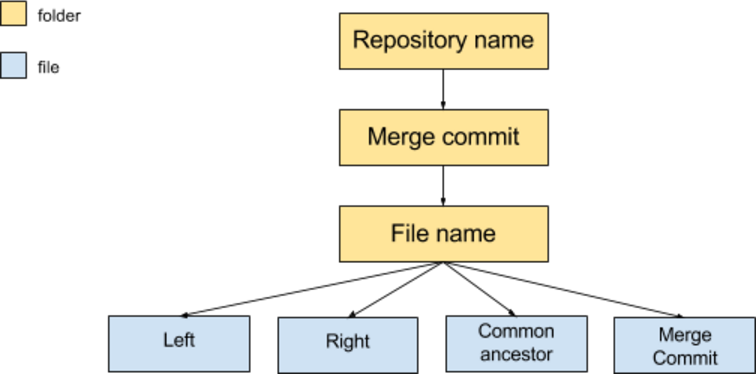
\includegraphics[width=0.45\linewidth, trim=3cm 11cm 3cm 11cm]{figure/conflicts.png}
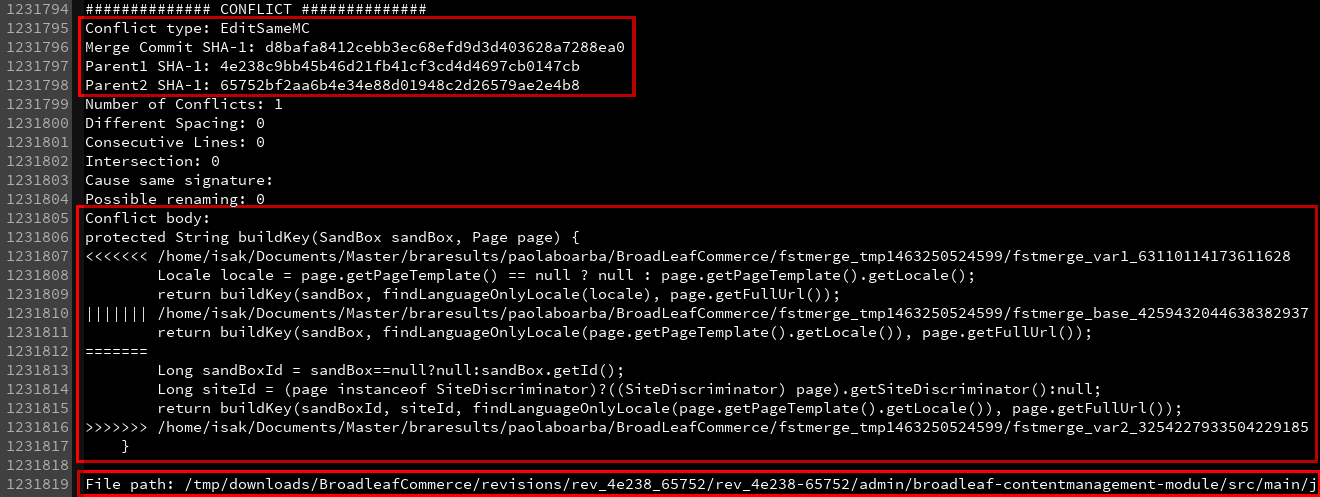
\includegraphics[width=400pt]{figure/screenshot.png}
\caption{Output data from Conflicts Analyzer}\label{fig:screenshot}
\end{figure}

From the “Conflict body” in the output, the name and signature of the conflicting function is parsed, as well as the parameter types that the function takes. The function body of the two versions in “Conflict body” is also parsed. This information is stored, and using the function name and the parameter types the function takes, the tool is able to parse the resolution function in the merge-commit by checking out the commit and reading the specified Java file from “File path”.

This information is then used to find the result from the resolution function in the merge-commit. The different versions of the function are extracted and saved. To filter out the conflicts that arose only due to different spacing or new lines on different places, each line in the extracted functions are trimmed and empty lines are removed. The conflicts in which the conflicting versions of the function thereafter are equal, are removed.

\subsection{Classifying Conflict Resolutions}
The automatic tool now classifies the merge-conflict resolutions according to the categories listed in Table \ref{table:pcategories2}. To do that, our tool first compares the left and right version of the function, to the function in the result. First they are checked for equality, ie. is the result equal to the left, right, both or none of the versions. This is used to see if they chose one version completely. By doing that, we can find out which categories that version belongs to.

\textbf{Superset.} To see if the result is a superset of the code in the left and right versions, first consider the following example of a superset:

Left version:
\lstset{language=Java,numbers=left,xleftmargin=2em,frame=single,framexleftmargin=1.5em}
\begin{lstlisting}[frame=single,breaklines=true,tabsize=2]
private int getValue(int index) {
	return (index >= values.size()) ? -1 : values[index];
}
\end{lstlisting}

Right version:
\lstset{language=Java,numbers=left,xleftmargin=2em,frame=single,framexleftmargin=1.5em}
\begin{lstlisting}[frame=single,breaklines=true,tabsize=2]
private int getValue(int index) {
	return values[index];
}
\end{lstlisting}
The left version contains all code from the right version plus a check for the index size. To detect that this is a superset it is not enough to compare them line by line. We solved this by instead considering the set of words in the code. All code in the left, right and result versions are therefore split into words and added to a hashset. A version is a superset if and only if the  that version’s set of words is equal to the set of all words in the left and right code.

\textbf{Intersection.} Similarly to how we detect a superset, we also consider the sets of words to detect whether a version is an intersection of the left and the right versions. A version is an intersection if and only if that version’s set of words is equal to the intersection of the sets of words in the left and right code.

\textbf{Recent.} Then, the tool extracts the commit date of the parents to see if the chosen version was the most recent one. The date of the commits are extracted using the command:
\lstset{language=Bash,numbers=left,xleftmargin=2em,frame=single,framexleftmargin=1.5em}
\begin{lstlisting}[frame=single,breaklines=true,tabsize=2]
git log -1 <hash> --format=%ci
\end{lstlisting}

\textbf{Keywords and if-statements.} Lastly, for each version of the method or constructor, we calculate the number of occurrences of each keyword and the number of if-statements (see Table \ref{table:pcategories2}). 
